In this section, we present some of the relevant metrics to measure similarities
between data points and explore where they can be used.

\subsection{Jaccard metric}
\label{subsect:jaccard_metric}
The Jaccard metric is a metric used to calculate the similarity between two sets
of values, it is defined as the size of the intersection set divided by the size
of the union set. It can be expressed with the following expression:
$$
    J(x, y) = \frac{x \cap y}{x \cup y}
$$
The figure \ref{fig:jaccard_metric} illustrates visually how the Jaccard metric
is computed.

\begin{figure}[h]
    \centering
    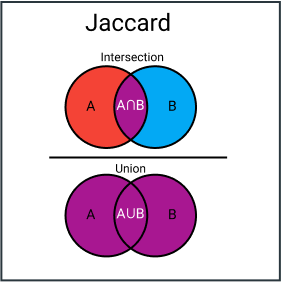
\includegraphics{state_of_the_art/metrics/jaccard-dist.png}
    \caption{Collision probability of LSH for the Jaccard metric}
    \label{fig:jaccard_metric}
\end{figure}

To get an estimation of the Jaccard metric using LSH, the hashing function is
defined as: $H(x) = min ( \pi (x_i) )$. It represents the index of the first row
in which is contained the minimum value of the data points (or the first occurrence of 1
in case of binary data) after a permutation $\pi$.

The collision probability between two data points following with this hashing
method is exactly equal to the Jaccard similarity \citep{yu_yun_2022}:
$$
    P( H(x) = H(y) ) = J(x, y) = \frac{|x\; \cap \;y|}{|x\; \cup \;y|}
$$


Jaccard similarity has found its use in multiple fields, we can mention its use
in text mining with the example of duplicate document detection, it can also be
used in e-commerce and recommendation systems to find similar customers via
their purchase history.

One obvious remark about the Jaccard metric is that it can be biased by the size
of the data, more precisely the large datasets increase significantly the size
of the union and thus reduce the similarity metric, so a dataset can have a
lower similarity metric with a dataset of large size than the one with a dataset
of smaller size even if they share more values.


\subsection{Hamming Metric}
\label{subsect:hamming_metric}
In case of binary data, this distance is expressed as the sum of the absolute
values of the element-to-element difference between two data vectors. More
generally the Hamming distance between two vectors is the number of distinct
values between them.

\begin{figure}[h]
    \centering
    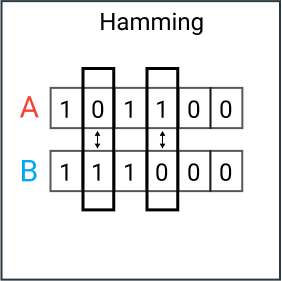
\includegraphics{state_of_the_art/metrics/hamming-dist.png}
    \caption{Hamming metric illustration}
    \label{fig:hamming_metric}
\end{figure}

To get an estimation of the Hamming metric using LSH, the hash function used is
$h(x) = x_i$ where $i$ is chosen randomly and $x_i$ represents the $i^{th}$
dimension of the data point $x$.

The probability of collision between two elements $x$ and $y$ is given by:
$$
    P(H(x) = H(y) ) = 1 - \frac{hamming(x,y)}{d}
$$

Where $hamming(x, y)$ is the hamming distance, and $d$ is the dimension of the data
points. This probability comes from the intuition that the number of indices
that verify $x_i = y_i$ is $n - d(x, y)$, and when this quantity is divided by
$n$, the total number of indices, we get the quantity described above.

It is obvious that this measure takes only into account the fact that the
values are different or equal, and doesn't pick attention to their values.

This Hamming metric is more fit to use when the magnitude is not an important
measure. Its main use is in the case we want to measure similarities or
differences between binary data vectors.

\subsection{Euclidean Metric}
\label{subsect:euclidean_metric}
It is the most commonly used metric as it represents the length of the segment
connecting the two points.
\begin{figure}[h]
    \centering
    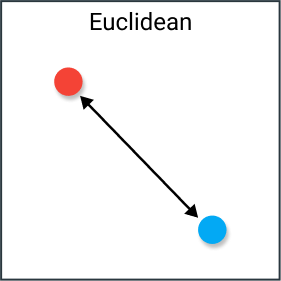
\includegraphics{state_of_the_art/metrics/euclidean-dist.png}
    \caption{Euclidean metric illustration}
    \label{fig:euclidean_metric}
\end{figure}

To get an estimation of the Euclidean metric using LSH, the used hashing
function is
$$
    h(x) = [\frac{a. x + b}{w}]
$$
Where $a$ is a $d$-dimension vector drawn from any Gaussian distribution and $b$
is drawn uniformly from $[0, w[$ where $w$ is the number of the hashing
functions.

This same hashing family can be used to get estimation of other metrics, it just
needs to change the distribution of the rotation vector $a$, we draw $a$ from
Levy distribution in the case of the Minkowski metric \citep{minkowski_2019},
and from Cauchy distribution in the case of the Manhattan metric
\citep{manhattan_2018}.

Contrary to the the Hamming metric, the Euclidean metric takes into account the
magnitude of the values of the data points. But on the other hand, it has a
limitation when dealing with data whose features are expressed in different
units, a limitation that can be resolved with normalizing the data. Moreover,
the values of this metric become less useful when the data has a lot of
features. And this comes from the fact that the geometric intuitions that we had
from the three-dimensional and the two-dimensional spaces are not often applied
in high dimensions. \citep{domingos_few_2012}
%explanation over here:
%https://stats.stackexchange.com/questions/99171/why-is-euclidean-distance-not-a-good-metric-in-high-dimensions


The Euclidean metric is more often used in algorithms like K-Mean where the data
dimension is low, and where the similarity between data points is gauged enough
with a straight forward distance.

\subsection{Angular metric}
\label{subsect:angular_metric}
The angular or cosine metric is simply the cosine measure between
the vectors of the two data points, it can also represent the inner product
between them if they are both normalized.

\begin{figure}[h]
    \centering
    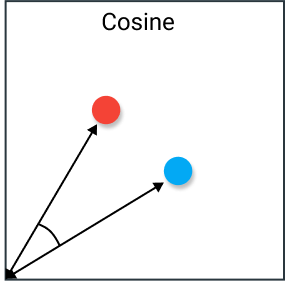
\includegraphics[height=0.4\textwidth]{state_of_the_art/metrics/angular-dist.png}
    \caption{Angular metric illustration}
    \label{fig:angular_metric}
\end{figure}

To get an estimation of the Angular metric using LSH, the hash function used
is defined as: $H(x)=\;sgn(a.x)$ where $sgn$ is the sign function, and $a$ is a
random $d$-dimensional vector drawn from any Gaussian distribution. The
illustration in the figure
\ref{fig:angular_illustration}
shows that the random drawn line (issued from a vector drawn from any Gaussian
distribution) splits the points in two groups, a group in the positive side and
another in the negative one.

The probability of having a collision between two elements is given by:
$$
    P(H(x)=H(y))=1- \frac{\theta}{\pi}
$$
The intuition behind this formula is that given an angle $\theta$ between two
vectors and a random line, this line has $\frac{\theta}{\pi}$ chance to cross
this angle, which means that it is also the chance to have these two vectors
separated by the line. The probability of collision will be: $1 -
    \frac{\theta}{\pi}$ \citep{jafari_lsh_2017}. The figure
\ref{fig:angular_collision_intuition} illustrates the meaning behind the
expression of the collision probability.


\begin{figure}[h]
    \centering
    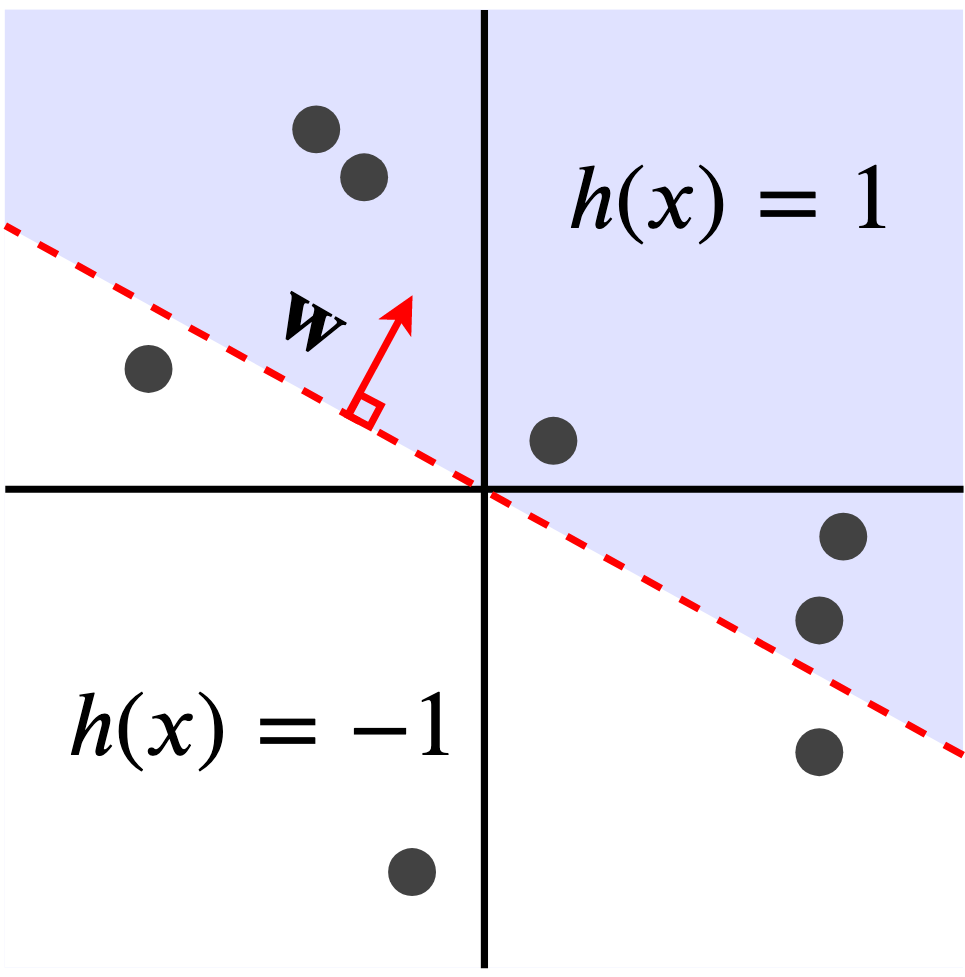
\includegraphics[width=0.25\textwidth, height=0.25\textheight]{state_of_the_art/metrics/angular-project.png}
    \caption{Angular metric estimation with LSH}
    \label{fig:angular_illustration}
\end{figure}

This metric has found its use in multiple cases, one of them is for similarity
estimation in text embeddings, as it doesn't present the limit of the euclidean
metric with high dimensional data. It can also be used for similarity estimation
between picture and fingerprint embeddings.

\begin{figure}[h]
    \centering
    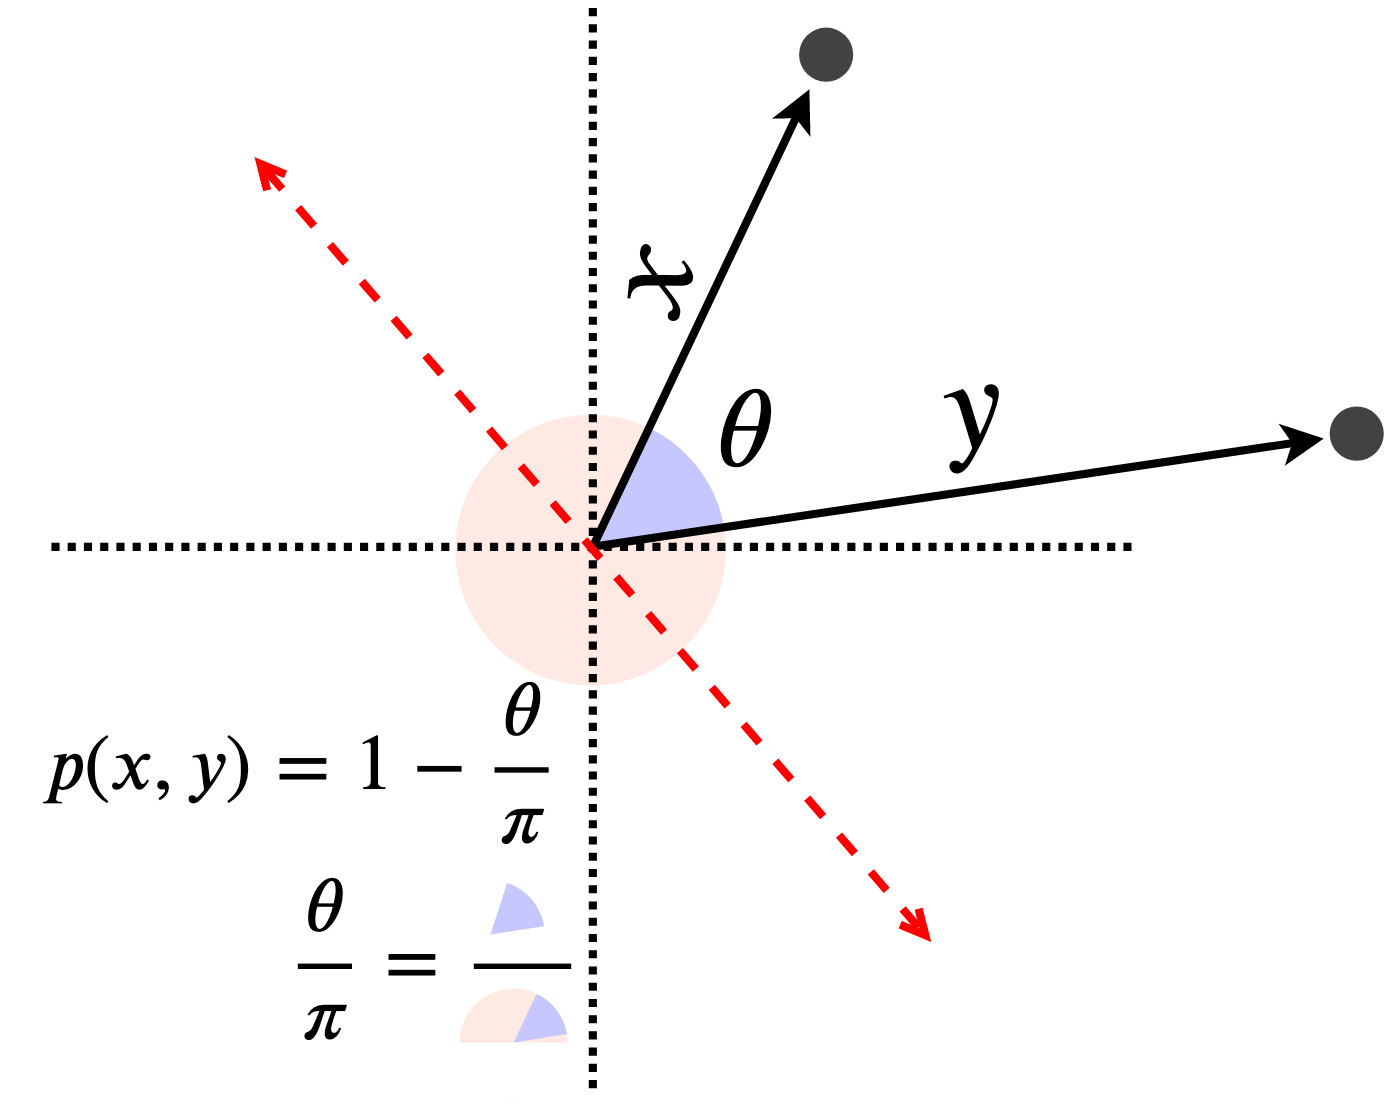
\includegraphics[width=\textwidth, height=0.35\textheight]{state_of_the_art/metrics/angular-collision.png}
    \caption{Collision probability of LSH for the angular metric}
    \label{fig:angular_collision_intuition}
\end{figure}
